\documentclass[12pt]{article}

\usepackage[utf8]{inputenc}
\usepackage[T1]{fontenc}
\usepackage{lmodern}
\usepackage{float}
\usepackage{amsmath}
\usepackage{latexsym,amsfonts,amssymb,amsthm,amsmath}
\usepackage{enumitem}
\usepackage{hyperref}
\usepackage{graphicx}
\usepackage{subcaption}
\usepackage{booktabs}
\graphicspath{{./images/}}

\setlength{\parindent}{0in}
\setlength{\oddsidemargin}{0in}
\setlength{\textwidth}{6.5in}
\setlength{\textheight}{8.8in}
\setlength{\topmargin}{0in}
\setlength{\headheight}{18pt}

\title{Pomiar Masy Włókna Żarówki}
\author{Kacper Kłos}

\begin{document}

\maketitle
W niniejszym doświadczeniu przedstawiamy metodę wyznaczania masy włókna żarówki wolframowej z wykorzystaniem sprzętu dostępnego w pracowni elektronicznej: multimetru, zasilacza, oscyloskopu oraz rezystora.  
Wyznaczymy najpierw tempo zmiany temperatury wolframu w badanej żarówce, a także moc dostarczaną i wytracaną przez żarówkę.  
Na podstawie tych danych dopasujemy prostą zależność, która – w połączeniu z wartościami materiałowymi wolframu (zaczerpniętymi z tabel) – pozwoli nam oszacować masę włókna.

\newpage
\section{Podstawy Teoretyczne}
W trakcie całego doświadczenia przyjmujemy, że rezystancje wszystkich elementów obwodu, poza żarówką, są stałe.  
Dla żarówki zakładamy, iż jej opór zmienia się liniowo z temperaturą w badanym zakresie i można go wyrazić następującym wzorem:
\begin{equation}
    R_w(T) = R_0 \bigl(1+\alpha\,(T - T_0)\bigr),
    \label{eq:resistance}
\end{equation}
gdzie:
\begin{itemize}
\item $R_w(T)$ – opór włókna przy temperaturze $T$,  
\item $R_0$ – opór włókna w ustalonej temperaturze referencyjnej $T_0$,  
\item $\alpha$ – współczynnik temperaturowy oporu (stała proporcjonalności dla wolframu).
\end{itemize}

Prąd przepływający przez żarówkę dostarcza do niej moc, która jest następnie wykorzystywana na:  
\begin{enumerate}
\item ogrzanie włókna (zwiększanie jego temperatury),  
\item straty ciepła (głównie w postaci wypromieniowanej energii).  
\end{enumerate}
Możemy zatem zapisać:
\begin{equation}
    P = P_s(T) + m\,c_w\,\frac{\Delta T}{\Delta t},
    \label{eq:mass}
\end{equation}
gdzie:  
\begin{itemize}
\item $P$ – moc dostarczana żarówce,  
\item $P_s(T)$ – moc wytracana (odprowadzana do otoczenia) przez żarówkę,  
\item $m$ – masa włókna,  
\item $c_w$ – ciepło właściwe wolframu,  
\item $\frac{\Delta T}{\Delta t}$ – tempo zmiany temperatury włókna w czasie.  
\end{itemize}

Zakładamy, że moc tracona przez żarówkę $P_s$ zależy tylko od temperatury włókna. Ze względu na to, że opór żarówki zależy liniowo od temperatury (zgodnie z równaniem \eqref{eq:resistance}), moc rozpraszana na żarówce jest wprost proporcjonalna do jej rezystancji.

Ponieważ znane są wartości tablicowe współczynników $c_w$ oraz $\alpha$ dla wolframu, do wyznaczenia masy włókna potrzebujemy doświadczalnie określić:  
\begin{itemize}
\item moc $P$ dostarczaną do żarówki,  
\item moc $P_s$ traconą przez włókno,  
\item zmianę temperatury w czasie $\frac{\Delta T}{\Delta t}$.  
\end{itemize}
Ostatecznie, korzystając z równania \eqref{eq:mass}, dopasowujemy krzywą pozwalającą wyznaczyć masę $m$. W tym celu pomiary dzielimy na dwie części.

\section{Układ Doświadczalny}
\subsection{Pomiar Stacjonarny}
W pierwszej części badamy zależność mocy oddawanej przez żarówkę od jej oporu. W tym celu korzystamy z układu z rys. \ref{fig:pomiar_stac}:
\begin{figure}[H]
    \centering
    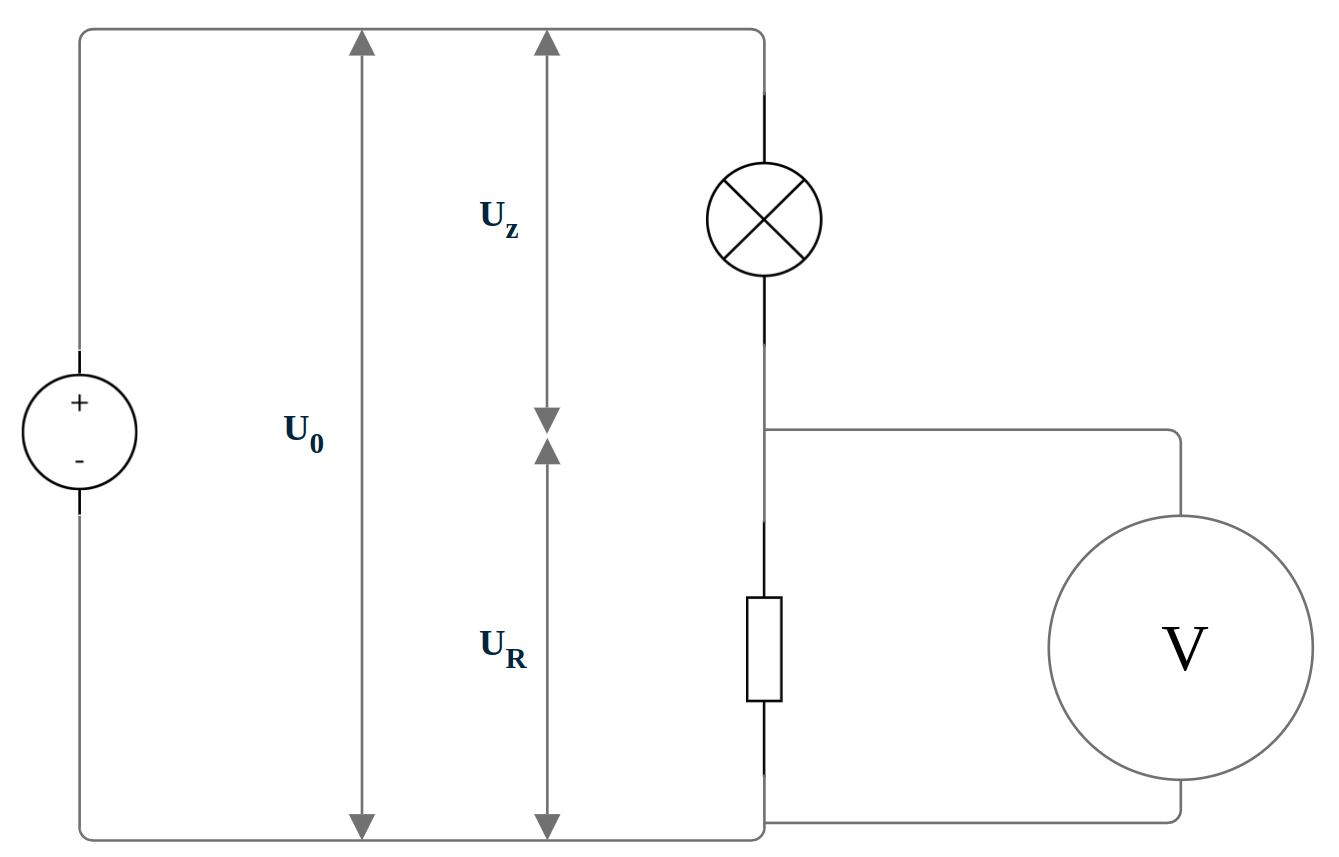
\includegraphics[scale=0.25]{static}
    \caption{Diagram układu używanego do pomiarów statycznych (źródło: \cite{diagram}).}
    \label{fig:pomiar_stac}
\end{figure}

Rozpisując równania na prądy i napięcia w tym układzie, otrzymujemy:

\begin{equation}
    P_s = P = U_z \cdot I = (U_0 - U_R) \frac{U_R}{R},
    \label{eq:power_dis}
\end{equation}
\begin{equation}
    R_w = \frac{U_0 - U_R}{U_R}\,R.
    \label{eq:bulb_resistance}
\end{equation}

Opory $R$ oraz $R_w$ łatwo zmierzyć przy pomocy multimetru. Z kolei do określenia $P_s$ wykorzystujemy fakt, że w stanie ustalonym (gdy temperatura przestaje się wyraźnie zmieniać,
a napięcie na żarówce stabilizuje się) moc dostarczana musi równać się mocy wytracanej, tj. $P_s = P$ zgodnie z \eqref{eq:power_dis}.

Dla niewielkich wartości oporu włókna (a tym samym małych wartości temperatury) zależność $P_s(R_w)$ jest w dobrym przybliżeniu liniowa, co motywuje dopasowanie funkcji:
\begin{equation}
    P_s = a\,R_w + b.
    \label{eq:power_line}
\end{equation}

\newpage

\subsection{Pomiary Dynamiczne}
W części dynamicznej układ jest analogiczny do użytego w pomiarach stacjonarnych, z tą różnicą, że zamiast woltomierza zastosowano oscyloskop (rys. \ref{fig:pomiar_dyn}):
\begin{figure}[H]
    \centering
    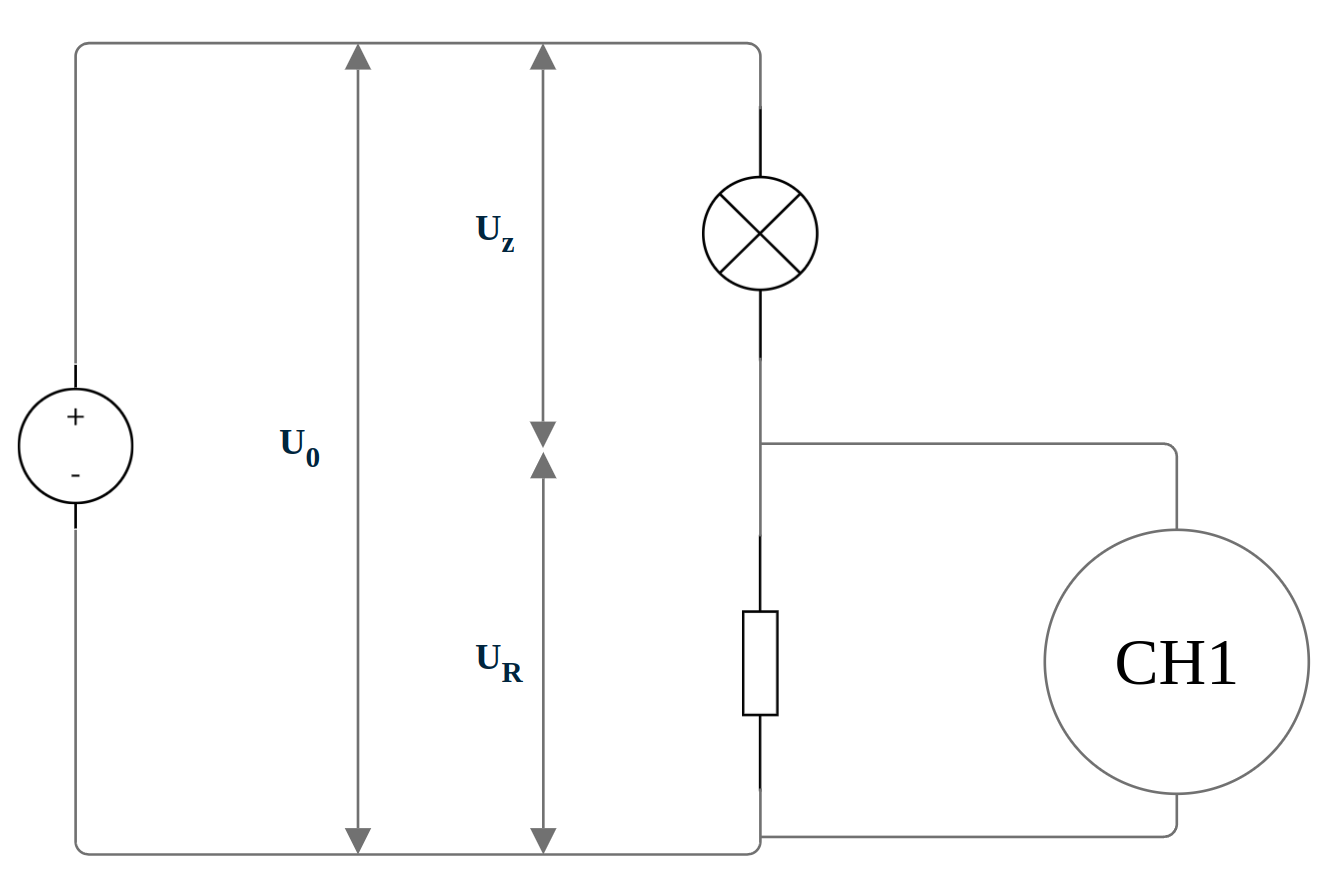
\includegraphics[scale=0.25]{dynamic}
    \caption{Diagram układu używanego do pomiarów dynamicznych (źródło: \cite{diagram}).}
    \label{fig:pomiar_dyn}
\end{figure}

Korzystając z równania \eqref{eq:resistance}, zauważamy, że przy zmianach oporu w czasie:
\begin{equation}
    \frac{\Delta T}{\Delta t} = \frac{1}{\alpha\,R_0}\,\frac{\Delta R_w}{\Delta t}.
    \label{eq:temp_der}
\end{equation}
Dla bardzo małych przedziałów czasowych $\frac{\Delta R_w}{\Delta t}$ możemy traktować jako pochodną $d R_w / d t$. Wówczas z \eqref{eq:bulb_resistance} wynika:
\begin{equation}
    \frac{d R_w}{d t} = -\,R\,\frac{U_0(t)}{U_R(t)^2}\,\frac{d U_R}{dt}.
    \label{eq:bulb_der}
\end{equation}
Przyjmując, że w krótkim czasie po przyłożeniu napięcia generatora $U_0(t)$ nie zmienia się istotnie (napięcie zasilania jest niemal stałe), możemy zastąpić pochodne różnicami i zapisać:
\begin{equation}
    \frac{\Delta T}{\Delta t} = -\,\frac{R\,U_0(t_0)}{\alpha\,R_0\,U_R(t_0)^2}\,\frac{\Delta U_R}{\Delta t},
    \label{eq:temp_delta}
\end{equation}
gdzie $t_0$ oznacza moment, w którym napięcie ustabilizowało się i zaczyna zachowywać się niemal liniowo.

Łącząc równania \eqref{eq:power_dis}, \eqref{eq:bulb_resistance}, \eqref{eq:temp_delta} z \eqref{eq:mass}, otrzymujemy ostatecznie:
\begin{equation}
    (U_0(t_0) - U_R(t_0))\frac{U_R(t_0)}{R}
    \;-\;
    a\,\frac{U_0(t_0) - U_R(t_0)}{U_R(t_0)}\,R
    \;-\; b
    \;=\;
    -\,m\,c_w\,\frac{R\,U_0(t_0)}{\alpha\,R_0\,U_R(t_0)^2}\,\frac{\Delta U_R}{\Delta t}.
    \label{eq:final}
\end{equation}
Dopasowując krzywą do powyższego równania, możemy wyznaczyć masę $m$ włókna.

\section{Wyniki Pomiarów}
W tej części przedstawiamy dane pomiarowe wraz z analizą niepewności.  
Korzystamy z następujących oznaczeń:  
\[
    \bar{x} \ \text{- średnia z wartości }x,\quad s_x \ \text{- niepewność statystyczna,}
\]
\[
    \delta x \ \text{- niepewność pomiarowa,}\quad u(x) \ \text{- niepewność całkowita.}
\]
Często też posługujemy się standardowym wzorem na propagację niepewności dla funkcji wielu zmiennych $f(x_1,\ldots,x_i)$:
\begin{equation}
    \delta f(x_1,\ldots,x_i)
    = \sqrt{\left(\frac{\partial f}{\partial x_1}\,\delta x_1\right)^2 + \dots + \left(\frac{\partial f}{\partial x_i}\,\delta x_i\right)^2}.
    \label{eq:error_propagation}
\end{equation}

\subsection{Opory}
Z instrukcji multimetru \cite{multimeter} wynika, że dla oporów w zakresie poniżej $200\,\Omega$ niepewność pomiarowa wynosi $\delta R =0.01\,\Omega + 3R\cdot10^{-4}$ gdzie R to zmierzony opór.
W oparciu o tą wiedze i wyniki pomiarów znajdujące się w tabeli \ref{tab:opory} wyznaczamy opory.
\begin{table}[H]
    \centering
    \begin{tabular}{c|cc}
        \toprule
        \textbf{Nr} & $R \, [\Omega]$ & $R_0 \, [\Omega]$ \\
        \midrule
        1 & 9{,}802  & 2{,}870 \\
        2 & 9{,}786  & 2{,}888 \\
        3 & 9{,}796  & 2{,}902 \\
        \bottomrule
    \end{tabular}
    \caption{Pomiary oporów dla rezystora ($R$) oraz żarówki w temperaturze referencyjnej ($R_0$).}
    \label{tab:opory}
\end{table}

Przyjmując wartości rzeczywiste jako średnie z pomiarów, otrzymujemy:
\[
    R = 9{,}795\,\Omega, \quad s_{R} = 0{,}0047\,\Omega, \quad \delta R = 0{,}0130\,\Omega, \quad u(R) = 0{,}014\,\Omega,
\]
\[
    R_0 = 2{,}887\,\Omega, \quad s_{R_0} = 0{,}0093\,\Omega, \quad \delta R_0 = 0{,}0109\,\Omega, \quad u(R_0) = 0{,}015\,\Omega,
\]

\newpage

\subsection{Pomiary Stacjonarne}
Dla wszystkich zarejestrowanych pomiarów przyjmujemy niepewność zasilacza według instrukcji \cite{generator}, tj. $0{,}05\% + 10\,\mathrm{mV}$.  
Za niepewność pomiaru woltomierza uznajemy maksymalne wahanie napięcia po jego ustabilizowaniu. Tabela \ref{tab:resistor_voltage} przedstawia uzyskane wyniki.
\begin{table}[H]
    \centering
    \begin{tabular}{c|cccc}
        \toprule
        Nr & $U_0 \,[V]$ & $U_R \,[V]$ & $\delta U_0 \,[V]$ & $\delta U_R \,[V]$ \\
        \midrule
        1  & 0{,}11  & 0{,}0805 & 0{,}011 & 0{,}0001  \\
        2  & 0{,}21  & 0{,}1547 & 0{,}011 & 0{,}0001  \\
        3  & 0{,}31  & 0{,}2255 & 0{,}011 & 0{,}0001  \\
        4  & 0{,}41  & 0{,}2907 & 0{,}011 & 0{,}0001  \\
        5  & 0{,}51  & 0{,}3472 & 0{,}011 & 0{,}0001  \\
        6  & 0{,}61  & 0{,}3921 & 0{,}011 & 0{,}0001  \\
        7  & 0{,}71  & 0{,}4284 & 0{,}011 & 0{,}0001  \\
        8  & 0{,}81  & 0{,}4618 & 0{,}011 & 0{,}0001  \\
        9  & 0{,}91  & 0{,}4944 & 0{,}011 & 0{,}0001  \\
        10 & 1{,}01  & 0{,}5270 & 0{,}011 & 0{,}0001  \\
        11 & 1{,}11  & 0{,}5592 & 0{,}011 & 0{,}0001  \\
        12 & 1{,}21  & 0{,}5908 & 0{,}011 & 0{,}0001  \\
        13 & 1{,}31  & 0{,}6221 & 0{,}011 & 0{,}0001  \\
        14 & 1{,}41  & 0{,}6524 & 0{,}011 & 0{,}0001  \\
        15 & 1{,}51  & 0{,}6823 & 0{,}011 & 0{,}0001  \\
        16 & 1{,}76  & 0{,}7548 & 0{,}011 & 0{,}0010  \\
        17 & 2{,}01  & 0{,}8228 & 0{,}012 & 0{,}0010  \\
        18 & 2{,}25  & 0{,}8881 & 0{,}012 & 0{,}0010  \\
        19 & 2{,}50  & 0{,}9512 & 0{,}012 & 0{,}0010  \\
        20 & 3{,}01  & 1{,}0717 & 0{,}012 & 0{,}0010  \\
        21 & 3{,}51  & 1{,}1843 & 0{,}012 & 0{,}0010  \\
        22 & 4{,}51  & 1{,}3915 & 0{,}013 & 0{,}0010  \\
        23 & 5{,}51  & 1{,}5800 & 0{,}013 & 0{,}0010  \\
        24 & 7{,}50  & 1{,}9144 & 0{,}014 & 0{,}0020  \\
        25 & 9{,}51  & 2{,}2113 & 0{,}015 & 0{,}0020  \\
        \bottomrule
    \end{tabular}
    \caption{Pomiary zależności napięcia na rezystorze $R$ od napięcia zasilającego $U_0$.}
    \label{tab:resistor_voltage}
\end{table}

Korzystając z równań \eqref{eq:bulb_resistance} i \eqref{eq:power_dis}, obliczamy niepewności $\delta R_w$ i $\delta P_s$ na drodze propagacji (zgodnie z \eqref{eq:error_propagation}).

\newpage

Wykres zależności mocy rozpraszanej przez żarówkę od jej oporu (z naniesionymi niepewnościami) przedstawiono na rys. \ref{fig:power_res_full}.
\begin{figure}[H]
    \centering
    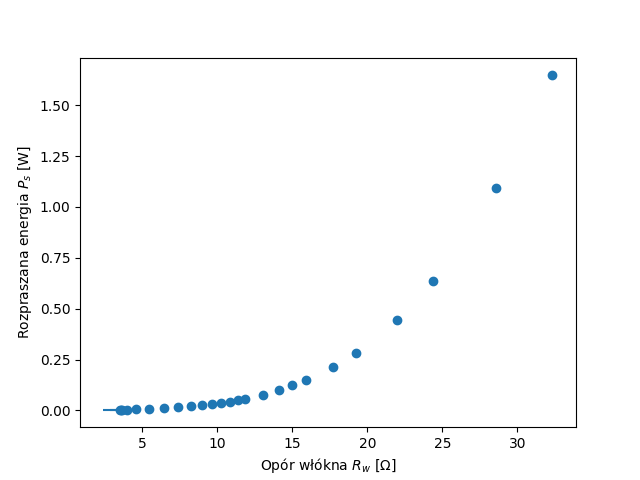
\includegraphics[scale=0.58]{pomiary_moc}
    \caption{Zależność mocy rozpraszanej przez żarówkę od jej oporu $R_w$, wraz z niepewnościami pomiarowymi.}
    \label{fig:power_res_full}
\end{figure}

Dla małych wartości oporu (przedział od ok. 1\,\(\Omega\) do 7\,\(\Omega\), czyli pomiary od 2 do 8) zależność ta jest prawie liniowa. W tym zakresie dopasowujemy funkcję \eqref{eq:power_line} metodą regresji ortogonalnej (rys. \ref{fig:power_res_line}).

\begin{figure}[H]
    \centering
    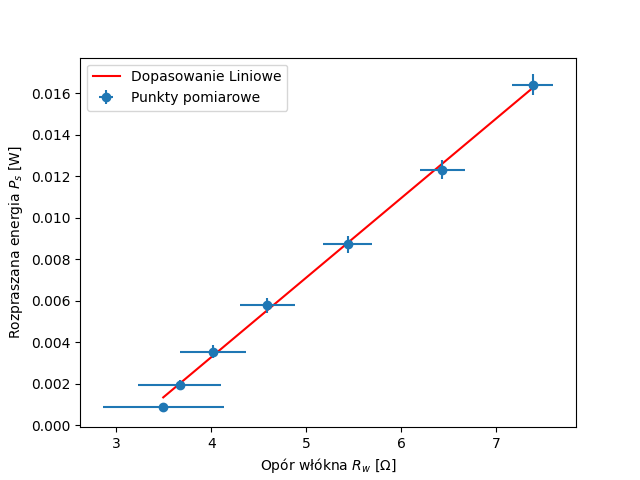
\includegraphics[scale=0.58]{pomiary_moc_linia}
    \caption{Dopasowanie liniowe do zależności $P_s(R_w)$ dla przedziału $R_w \in [1\,\Omega,\; 7\,\Omega]$.}
    \label{fig:power_res_line}
\end{figure}
Wyniki dopasowania to:
\[
    a = 0{,}00383 \ W\Omega^{-1}, \quad u(a) = 0{,}00008 \ W\Omega^{-1}, \qquad
    b = -\,0{,}0121 \ W, \quad u(b) = 0{,}0005 \ W.
\]
Na tej podstawie można oszacować opór spoczynkowy żarówki, przyjmując, że w chwili $P_s = 0$ (brak emisji energii) $R_w = R_0$:
\begin{equation}
    R_0 = -\frac{b}{a}, 
    \quad
    \delta R_0^2 = \left(\frac{u(a)}{b}\right)^2 + \left(\frac{a}{b^2}u(b)\right)^2.
\end{equation}
Podstawiając dane, otrzymujemy:
\[
    R_0 = 3{,}14\,\Omega, \quad u(R_0) = 0{,}13\,\Omega.
\]
Jest to wartość nieco odbiegająca od rezultatu otrzymanego bezpośrednio z pomiarów multimetrem (różnica <\,10\%). 
W dalszej analizie korzystamy jednak z wartości pomierzonej multimetrem, ze względu na jej mniejszą niepewność oraz bardziej zaufaną metodologię (trudno przewidzieć co dzieje się przey ciągłym zmniejszaniu oporu włókna $R_w$).

\subsection{Pomiary Dynamiczne}
W tej części badamy zależność $U_R(t)$ tuż po przyłożeniu napięcia $U_0$. Na oscyloskopie rejestrujemy krótki przedział czasowy zaraz po „skoku” napięcia, dopasowujemy prostą do $U_R(t)$ i wyznaczamy jej współczynnik kierunkowy (pochodną). W tabeli \ref{tab:lines_data} zestawiono zarejestrowane napięcia w seriach pomiarowych.

\begin{table}[H]
    \centering
    \begin{tabular}{c|c|ccccc|c}
        \toprule
        $U_0 \,[V]$ & $\delta U_0 \,[V]$ & \multicolumn{5}{c}{Serie Pomiarowe} & $\delta U_R \,[V]$ \\
        \midrule
        & & \multicolumn{5}{c}{$U_R \,[V]$} & \\
        10{,}1  & 0{,}016 & 6{,}760  & 6{,}740  & 6{,}680  & 6{,}640  & 6{,}600 & 0{,}12 \\
                &         & \textit{3{,}040}  & \textit{3{,}240}  & \textit{3{,}560}  & \textit{3{,}920}  & \textit{4{,}080} &   \\
                &         & \multicolumn{5}{c}{\textbf{t [ms]}} & \\[6pt]
        \midrule
        9{,}01  & 0{,}015 & 6{,}130  & 6{,}070  & 6{,}010  & 5{,}970  & 5{,}930 & 0{,}12 \\
                &         & \textit{7{,}160}  & \textit{7{,}800}  & \textit{8{,}280}  & \textit{8{,}760}  & \textit{9{,}120} & \\
                &         & \multicolumn{5}{c}{\textbf{t [ms]}} & \\[6pt]
        \midrule
        8{,}00  & 0{,}014 & 5{,}600  & 5{,}540  & 5{,}500  & 5{,}420  & 5{,}360 & 0{,}10 \\
                &         & \textit{5{,}600}  & \textit{6{,}400}  & \textit{7{,}000}  & \textit{8{,}000}  & \textit{9{,}000} & \\
                &         & \multicolumn{5}{c}{\textbf{t [ms]}} & \\[6pt]
        \midrule
        7{,}01  & 0{,}014 & 4{,}600  & 4{,}560  & 4{,}520  & 4{,}480  & 4{,}440 & 0{,}08 \\
                &         & \textit{7{,}400}  & \textit{8{,}200}  & \textit{9{,}000}  & \textit{9{,}800}  & \textit{10{,}60} & \\
                &         & \multicolumn{5}{c}{\textbf{t [ms]}} & \\[6pt]
        \midrule
        6{,}01  & 0{,}014 & 4{,}330  & 4{,}270  & 4{,}230  & 4{,}190  & 4{,}130 & 0{,}08 \\
                &         & \textit{8{,}400}  & \textit{10{,}00}  & \textit{11{,}60}  & \textit{12{,}80}  & \textit{14{,}80} & \\
                &         & \multicolumn{5}{c}{\textbf{t [ms]}} & \\[6pt]
        \midrule
        5{,}01  & 0{,}013 & 3{,}170  & 3{,}130  & 3{,}110  & 3{,}090  & 3{,}030 & 0{,}06 \\
                &         & \textit{10{,}00}  & \textit{11{,}60}  & \textit{13{,}20}  & \textit{14{,}80}  & \textit{16{,}40} & \\
                &         & \multicolumn{5}{c}{\textbf{t [ms]}} & \\[6pt]
        \midrule
        4{,}01  & 0{,}013 & 3{,}000  & 2{,}980  & 2{,}960  & 2{,}880  & 2{,}840 & 0{,}05 \\
                &         & \textit{12{,}00}  & \textit{14{,}40}  & \textit{16{,}40}  & \textit{24{,}80}  & \textit{30{,}00} & \\
                &         & \multicolumn{5}{c}{\textbf{t [ms]}} & \\[6pt]
        \midrule
        3{,}01  & 0{,}012 & 1{,}844  & 1{,}830  & 1{,}816  & 1{,}804  & 1{,}792 & 0{,}02 \\
                &         & \textit{20{,}40}  & \textit{23{,}60}  & \textit{26{,}00}  & \textit{29{,}20}  & \textit{32{,}80} & \\
                &         & \multicolumn{5}{c}{\textbf{t [ms]}} & \\[6pt]
        \midrule
        2{,}01  & 0{,}012 & 1{,}418  & 1{,}410  & 1{,}390  & 1{,}386  & 1{,}383 & 0{,}01 \\
                &         & \textit{26{,}40}  & \textit{31{,}20}  & \textit{38{,}80}  & \textit{42{,}80}  & \textit{46{,}00} & \\
                &         & \multicolumn{5}{c}{\textbf{t [ms]}} & \\[6pt]
        \bottomrule
    \end{tabular}
    \caption{Serie pomiarowe napięcia $U_R(t)$ tuż po ustabilizowaniu się wartości $U_0$. W nawiasach kursywą podano czasy w ms.}
    \label{tab:lines_data}
\end{table}

Po dopasowaniu prostych metodą najmniejszych kwadratów do każdej serii otrzymujemy współczynnik kierunkowy $\frac{dU_R}{dt}$ oraz wartość $U_R(t_0)$ (pierwszy punkt po ustaleniu napięcia). Dane zestawiono w tabeli \ref{tab:dynamic_data}:

\begin{table}[H]
    \centering
    \begin{tabular}{cc|cc|cc}
        \toprule
        $U_0(t_0)\,[V]$ & $\delta U_0(t_0)\,[V]$ & $U_R(t_0)\,[V]$ & $\delta U_R(t_0)\,[V]$ & $\frac{dU_R}{dt}\,[V/ms]$ & $\delta\bigl(\frac{dU_R}{dt}\bigr)$ \\
        \midrule
        10{,}1  & 0{,}016 & 6{,}760  & 0{,}12   & -0{,}151   & 0{,}0010 \\
        9{,}01  & 0{,}015 & 6{,}130  & 0{,}12   & -0{,}102   & 0{,}0040 \\
        8{,}00  & 0{,}014 & 5{,}600  & 0{,}10   & -0{,}0713  & 0{,}0019 \\
        7{,}01  & 0{,}014 & 4{,}600  & 0{,}08   & -0{,}050   & 0{,}0000 \\
        6{,}01  & 0{,}014 & 4{,}330  & 0{,}08   & -0{,}031   & 0{,}0010 \\
        5{,}01  & 0{,}013 & 3{,}170  & 0{,}06   & -0{,}020   & 0{,}0030 \\
        4{,}01  & 0{,}013 & 3{,}000  & 0{,}05   & -0{,}0090  & 0{,}0003 \\
        3{,}01  & 0{,}012 & 1{,}844  & 0{,}02   & -0{,}0043  & 0{,}0003 \\
        2{,}01  & 0{,}012 & 1{,}418  & 0{,}01   & -0{,}00190 & 0{,}00019 \\
        \bottomrule
    \end{tabular}
    \caption{Zestawienie napięć $U_0(t_0)$, $U_R(t_0)$ i współczynników kierunkowych $\frac{dU_R}{dt}$ po dopasowaniu do serii pomiarowych.}
    \label{tab:dynamic_data}
\end{table}
Za niepewność każdego $U_R(t_0)$ przyjmujemy największe zaobserwowane wychylenie napięcia w danej serii. Zakładamy, że czas (odczyt z oscyloskopu) jest zmierzony z pomijalną niepewnością.

\section{Masa Włókna}
Dla wygody definiujemy zmienne pomocnicze, wynikające z równania \eqref{eq:final}:
\begin{equation}
    X = -\,\frac{R\,U_0(t_0)}{\alpha\,R_0\,U_R(t_0)^2}\,\frac{\Delta U_R}{\Delta t},
\end{equation}
\begin{equation}
    Y = \;(U_0(t_0) - U_R(t_0))\frac{U_R(t_0)}{R}
    \;-\;a\,\frac{U_0(t_0) - U_R(t_0)}{U_R(t_0)}\,R
    \;-\; b.
\end{equation}
Wówczas równanie \eqref{eq:final} przyjmuje postać:
\begin{equation}
    Y = m\,c_w\,X.
    \label{eq:final_line}
\end{equation}
Do obliczeń potrzebujemy jeszcze wartości $\alpha$ dla wolframu. Korzystamy z danych \cite{heat_resist}, przyjmując $\alpha = 4{,}5 \times 10^{-3}\,K^{-1}$.

Na rys. \ref{fig:final_graph} przedstawiono punktową zależność $Y(X)$ wraz z dopasowaną linią prostą.
\begin{figure}[H]
    \centering
    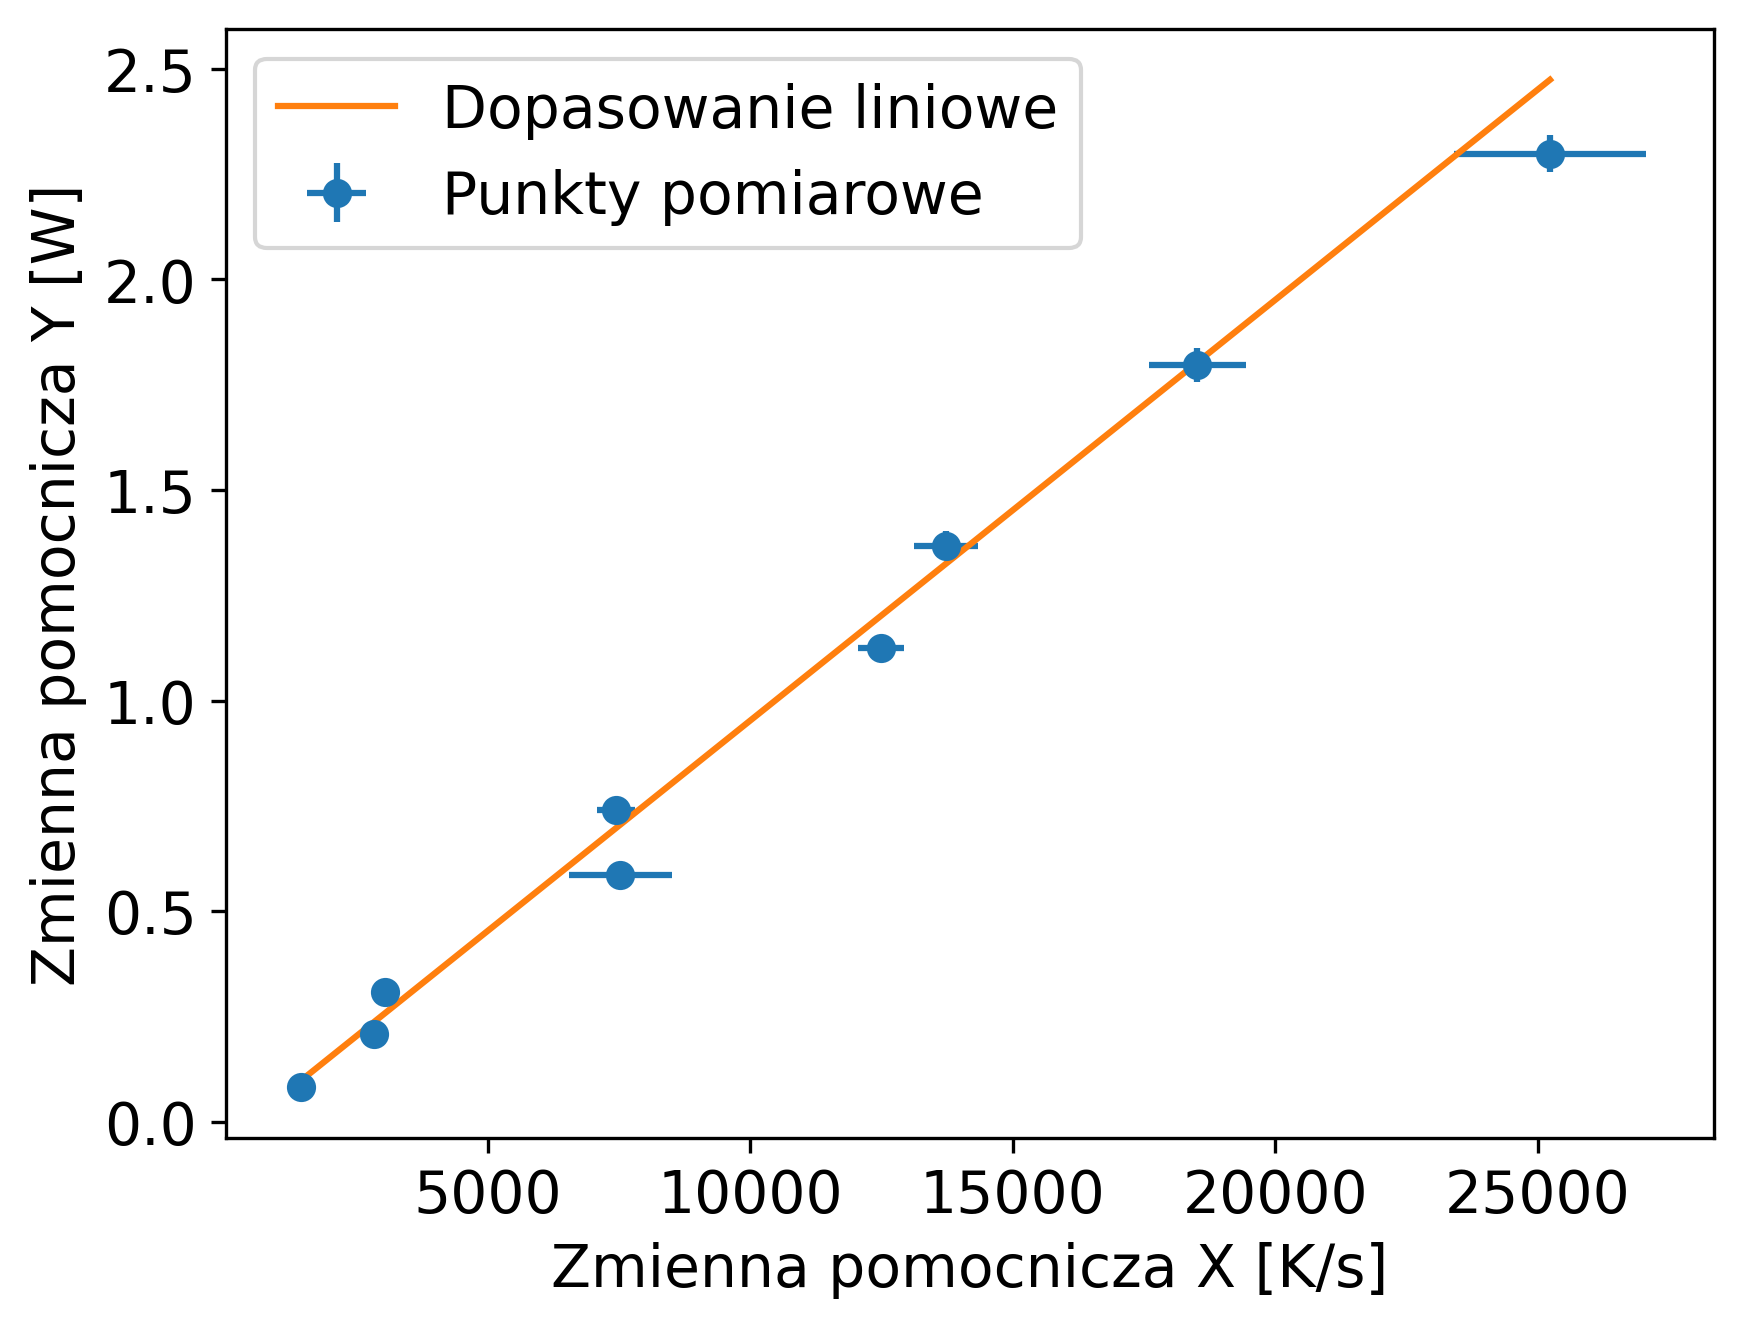
\includegraphics[scale=0.7]{final_graph}
    \caption{Zależność $Y$ od $X$ z równania \eqref{eq:final_line}, wraz z liniowym dopasowaniem do danych.}
    \label{fig:final_graph}
\end{figure}
Wynik dopasowania daje:
\[
    m\,c_w = 1{,}0\times 10^{-5}\,\mathrm{J/K}, 
    \quad
    u(m\,c_w) = 0{,}5\times 10^{-5}\,\mathrm{J/K}.
\]
Wykorzystując wartość ciepła właściwego wolframu $c_w = 144\,\mathrm{J/(kg\,K)}$ \cite{heat_capacity}, otrzymujemy ostatecznie:
\[
    m =0{,}69\,\mathrm{mg},
    \quad
    u(m) = 0{,}04\,\mathrm{mg}.
\]

\newpage

\section{Podsumowanie}
W przedstawionym doświadczeniu staraliśmy się wyznaczyć masę włókna żarówki wolframowej. Na początku określiliśmy opór żarówki oraz rezystora, wykonując kilka pomiarów miernikiem uniwersalnym (tabela~\ref{tab:opory}). Otrzymaliśmy wartości $R_{0} = 2{,}887 \pm 0{,}015\,\Omega$ dla żarówki oraz $R = 9{,}795 \pm 0{,}014\,\Omega$ dla rezystora.

Następnie zmierzyliśmy napięcie na oporniku w zależności od napięcia zasilacza, aby dopasować zależność liniową dla małych napięć do wzoru~\ref{eq:power_dis}. Z tabeli~\ref{tab:resistor_voltage} wybraliśmy kilka pierwszych punktów, w których obserwowaliśmy zależność liniową, i dopasowaliśmy krzywą widoczną na rys.~\ref{fig:power_res_line}, uzyskując wartości współczynników $a=0{,}00383 \pm 0{,}00008\,W\,\Omega^{-1}$ oraz $b=-0{,}0121 \pm 0{,}0005\,W$.

Kolejno, dopasowaliśmy prostą (tabela~\ref{tab:lines_data}) do napięcia na rezystorze w funkcji czasu dla kilku wartości napięcia ustawionych na generatorze (tabela~\ref{tab:dynamic_data}), tuż po zamknięciu układu. Wszystkie otrzymane wielkości wprowadziliśmy do równania~\eqref{eq:final}, do którego również dopasowaliśmy prostą pozwalającą nam wyznaczyć końcowy wynik masy włókna żarówki: $m=0{,}69\pm0{,}04\,\mathrm{mg}$.


\newpage
\begin{thebibliography}{5}

\bibitem{diagram}
\url{https://www.smartdraw.com/circuit-diagram/}, tworzenie diagramów układów elektrycznych.

\bibitem{multimeter}
\url{http://pracownie1.fuw.edu.pl/przyrzady/Multimetr_Rigol_DM3058_UserGuide_EN.pdf}, instrukcja multimetru Rigol DM3058.

\bibitem{generator}
\url{http://pracownie1.fuw.edu.pl/przyrzady/Zasilacz_Rigol_DP800_UserGuide_EN.pdf}, instrukcja zasilacza Rigol DP832.

\bibitem{heat_resist}
Giancoli, Douglas C., \emph{Physics}, 4th Ed.

\bibitem{heat_capacity}
A. Łopion, P. Węgrzyn, P. Fita, \emph{Żarówka}.

\end{thebibliography}

\end{document}

